\section{Problem Setup}

\subsection{Model-Heterogeneous CLE}

We consider clients \(k\in\{1,\ldots,K\}\), each with a private dataset and classifier \(f_k\); architectures need not match across clients. Our controlled implementation uses four heterogeneous clients with ResNet10, ResNet12, ShuffleNet, and MobileNetV2 on a CIFAR-10 private task. We use two complementary protocols. The \textbf{mechanism protocol} uses a Dirichlet label partition with concentration \(\alpha=0.5\), corrupts every private training image (\(\rho=1\)), and sets a strong class--operator association. The \textbf{main evaluation protocol} uses \(\alpha=1.0\), applies corruption to a fixed half of the private samples (\(\rho=0.5\)), and varies the association strength. The former maximizes identifiability of the shortcut mechanism; the latter jointly evaluates DSA and task utility under a clean--corrupted mixture. Results from the two protocols are not pooled into one leaderboard.

Let \(Y\) denote the task class, \(O\) a concrete corruption operator, and \(F=\pi(O)\) its coarse corruption family. CLE-HFL introduces client-specific class dependence,

\[
P_k(O=o\mid Y=c)\neq P_k(O=o),
\]

with a pre-registered client-specific binding

\[
b_k:\mathcal C\rightarrow\mathcal O.
\]

For \(M=|\mathcal O_{\mathrm{seen}}|\) seen operators, the training operator is sampled according to

\[
P_k(O=o\mid Y=c)
=\frac{1-\gamma_{\mathrm{CLE}}}{M}
+\gamma_{\mathrm{CLE}}\,\mathbf 1\{o=b_k(c)\}.
\]

The control setting uses \(\gamma_{\mathrm{CLE}}=0\), while the strong-binding condition uses \(\gamma_{\mathrm{CLE}}=0.9\), making \(b_k(c)\) a strong but non-deterministic dominant operator for class \(c\). The main evaluation protocol additionally includes \(\gamma_{\mathrm{CLE}}=0.5\). Its corruption mask is held fixed across all three values of \(\gamma_{\mathrm{CLE}}\), separating exposure to corruption from concentration along the binding. The paired evaluation uses 1,000 semantic sources, 15 operators, four clients, and corruption severity 3.

CLE-v2 and DSA use operator-level bindings, whereas the deployable intervention remains coarse family-level. PEW predicts a corruption-family proxy, and BER groups private fit samples by task class and that proxy. The training rule never reads private operator metadata. Operator identities and the binding map are reserved for controlled CLE construction, sealed DSA evaluation, and non-deployable Oracle audits.

\subsection{Information Separation}

Private data are separated by role. The \textbf{private fit} subset produces local gradients and BER group counts. A \textbf{private audit} subset may support strict communication routing but does not produce local-training gradients. The \textbf{final task test} is used only for frozen utility reporting. The \textbf{paired operator grid} is used only after training for DSA. Public data support PEW training or pre-existing communication without private-task ground-truth leakage.

During training, the method reads neither private true operator IDs nor true corruption families, evaluation severity, seen/unseen flags, or the paired evaluation binding. The frozen binding is read only after model sealing to compute DSA. This separation keeps the target-aligned diagnostic outside optimization, routing, tuning, and model selection.

\begin{figure*}[t]
\centering
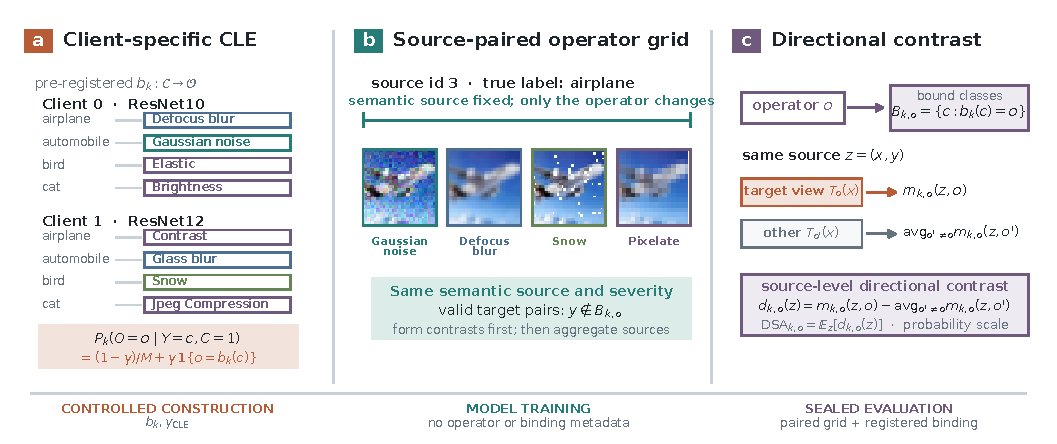
\includegraphics[width=\textwidth,keepaspectratio]{figures/fig_cle_paired_dsa_v4.pdf}
\caption{CLE construction and paired diagnosis. (a) Examples from two of the four heterogeneous clients illustrate distinct registered class--operator bindings; the operator draw is conditional on a sample being corrupted. (b) Four of the 15 operator views of one semantic source illustrate the fixed-source, fixed-severity grid. (c) DSA compares predictive mass assigned to operator-bound classes against the other views, using only valid targets with $y\notin B_{k,o}$. Operator identities and the binding remain outside model training.}
\label{fig:cle-paired-dsa}
\end{figure*}

\section{Paired Diagnosis and Identification}

\subsection{Directional Shortcut Alignment}

For source \(z=(x,y)\), let \(T_o(x)\) be a semantic-preserving corruption transformation. For client \(k\) and operator \(o\), define the classes bound to that operator during training:

\[
B_{k,o}=\{c:b_k(c)=o\}.
\]

We evaluate only source--operator pairs for which \(y\notin B_{k,o}\), avoiding a trivial contribution from the source's true class. Define bound probability mass

\[
m_{k,o}(z,o')=\sum_{c\in B_{k,o}}p_k(c\mid T_{o'}(x)).
\]

The source-level directional contrast is

\[
d_{k,o}(z)=m_{k,o}(z,o)
-\frac{1}{|\mathcal O|-1}\sum_{o'\neq o}m_{k,o}(z,o'),
\]

and

\[
\operatorname{DSA}_{k,o}=\mathbb E_z[d_{k,o}(z)].
\]

Pooled DSA equally averages valid operator-level values and then client-level values:

\[
\operatorname{DSA}_{\mathrm{pool}}
=\frac1K\sum_{k=1}^{K}
\frac1{|\mathcal O_k^{\mathrm{valid}}|}
\sum_{o\in\mathcal O_k^{\mathrm{valid}}}\operatorname{DSA}_{k,o}.
\]

DSA lies on a probability scale: a value of \(0.12\) means roughly a 12-percentage-point directional difference in predictive mass, not a \(0.12\)-point accuracy difference.

DSA asks a specific question: for the same semantic source, does applying operator \(o\) move probability toward the classes associated with \(o\) during this client's training, relative to other operators? Under the stated assumptions, this is a binding-direction operator-response contrast rather than a reconstruction of the model's full internal causal mechanism.

Figure~\ref{fig:cle-paired-dsa} illustrates the fixed-source operator comparison and its registered direction. The identification properties and proxy boundary are developed below.

\subsection{Paired Cancellation and Binding Specificity}

The following cancellation property is a statement about the paired estimand, not a generative model of the network. Write

\[
m_{k,o}(z,o')=s_{k,o}(z)+r_{k,o}(z,o'),
\]

where \(s_{k,o}(z)\) is an operator-invariant source term and \(r_{k,o}\) is an operator-dependent response. Then

\[
d_{k,o}(z)=r_{k,o}(z,o)
-\frac{1}{|\mathcal O|-1}\sum_{o'\neq o}r_{k,o}(z,o'),
\]

so the operator-invariant source term cancels exactly. DSA therefore isolates the operator-dependent part of the paired response along the pre-registered binding direction. Semantic validity of the transformations and relevance beyond the evaluated distribution remain separate assumptions.

To test binding specificity, we preserve the number of classes assigned to each operator but randomly permute the binding and recompute DSA on the same prediction cache. Under the primary strong-CLE HFL checkpoint, true-binding DSA is \(0.119644\), whereas the shuffled-binding null has p95 \(=0.029559\) with permutation \(p=0.000999\). The gap between the true binding and this null is evidence that the measured response follows the training association rather than only a generic operator-to-class preference.

\subsection{Why Consistency and Proxy Scores Are Insufficient}

Within-operator consistency and cross-operator directional invariance are different objects. If multiple predictive views around the same corrupted observation are identical, their JSD is zero; predictions can nevertheless differ systematically across corruption operators. In a fixed-cache construction, within-operator JSD is zero while DSA remains \(0.119644\). Thus,

\[
\begin{aligned}
&\text{within-operator consistency}\\
&\qquad\not\Rightarrow\qquad
\text{cross-operator directional invariance}.
\end{aligned}
\]

JSD and DSA therefore answer different questions: local consistency around a corrupted view versus cross-operator alignment with the training binding.

The same separation yields a proxy non-identifiability result. Let \(Z\) be a proxy environment predicted by PEW and \(E\) the latent true corruption environment. Define

\[
\mathcal D(A,B)=TV(P_{A,B},P_AP_B).
\]

With no constraint on the error channel \(P(Z\mid E,Y)\), a fixed observable \(P(Y,Z)\) can correspond to one latent world with \(\mathcal D(Y,E)=0\) and another with

\[
\mathcal D(Y,E)=1-\sum_eP(E=e)^2>0.
\]

Thus \(P(Y,Z)\) alone does not identify true environment dependence. A conditional bridge remains valid under sample-wise coupling:

\[
\mathcal D_Q(Y,E)\le
\mathcal D_Q(Y,Z)+2\epsilon_Q,
\qquad
\epsilon_Q=P_Q(Z\neq E).
\]

In the audited BER effective distribution, the PEW family error is \(0.507\)--\(0.575\), so the numerical upper bound becomes trivial after truncation at 1.0. This does not imply that PEW is useless for training; it means that its observable statistics cannot certify true CLE mitigation. That claim is evaluated with paired DSA instead. Appendix A gives the constructive proof and algebraic checks.

\subsection{Statistical Unit}

The independent evaluation unit is the \textbf{semantic source}. Multiple operator views of one source share content, so we first form source-level contrasts and then use a source-clustered bootstrap. These intervals quantify evaluation-source uncertainty conditional on the trained checkpoint; training-seed, partition, binding-map, model-selection, and cross-dataset uncertainty require separate analyses.

\section{Taxonomy-Assisted Local Mitigation}

\subsection{Public Environment Witness}

The \textbf{Public Environment Witness (PEW)} is trained only on public carrier images with programmatically generated corruption supervision. It is frozen as a \textbf{coarse family-level witness} over

\[
\{\text{clean},\text{noise},\text{blur},\text{weather},\text{digital},\text{unknown}\}.
\]

For each private fit sample, PEW produces a hard pseudo-environment \(\hat e_i\). Its semantics come from a predefined corruption-family taxonomy learned from public synthetic corruptions, while private true operator and family metadata remain unavailable at training time. PEW is therefore \textbf{taxonomy-assisted}; architecture and optimizer details appear in Appendix B because the witness supplies side information rather than serving as the architectural contribution.

The two levels of granularity serve different roles: CLE-v2 construction and DSA evaluation are operator-level, whereas PEW and BER use coarse family-level pseudo-environments. Appendix C uses true operator metadata only in a non-deployable Oracle audit; the deployable witness remains family-level.

Figure~\ref{fig:pew-ber-execution} shows how the frozen public witness supplies the class-conditional groups used by the local risk below.

\begin{figure*}[t]
\centering
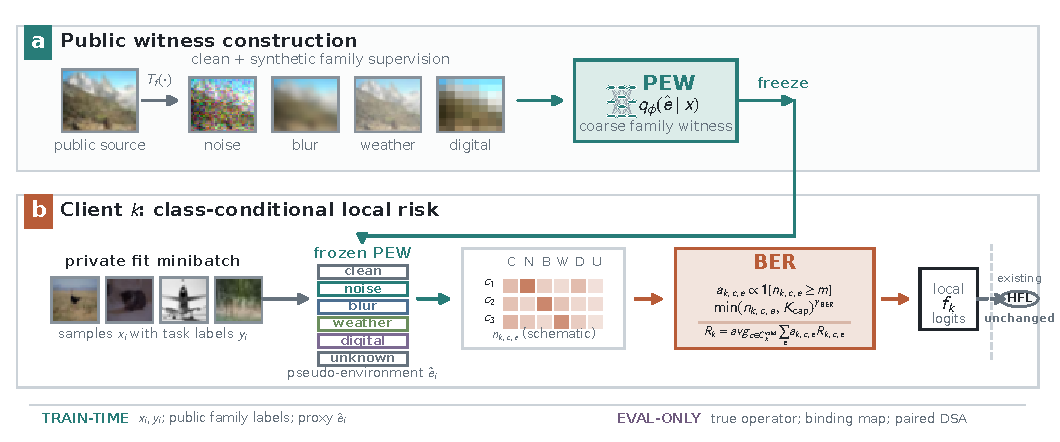
\includegraphics[width=\textwidth,keepaspectratio]{figures/fig_pew_ber_execution_v3.pdf}
\caption{PEW+BER execution. Public clean images and synthetic corruption-family labels train the witness, which is then frozen for private fit inference. Its coarse pseudo-environments include clean, noise, blur, weather, digital, and unknown. BER computes class-conditional support and balances valid environment risks without changing the existing HFL communication. The thumbnail transformations and support-cell shading are schematic illustrations; true private operator and family labels are not training inputs.}
\label{fig:pew-ber-execution}
\end{figure*}

\subsection{Balanced Environment Risk}

For client \(k\), task class \(c\), and pseudo-environment \(e\), define

\[
n_{k,c,e}=\#\{i:y_i=c,\hat e_i=e\}.
\]

\[
R_{k,c,e}=\frac1{n_{k,c,e}}\sum_{i:y_i=c,\hat e_i=e}\ell_i.
\]

BER assigns class-conditional environment weight

\[
a^{(\gamma_{\mathrm{BER}})}_{k,c,e}
=
\frac{
\mathbf 1[n_{k,c,e}\ge m]
\min(n_{k,c,e},K_{\mathrm{cap}})^{\gamma_{\mathrm{BER}}}
}{
\sum_{e'}
\mathbf 1[n_{k,c,e'}\ge m]
\min(n_{k,c,e'},K_{\mathrm{cap}})^{\gamma_{\mathrm{BER}}}
},
\]

with the frozen Formal configuration

\[
\gamma_{\mathrm{BER}}=0.5,\qquad K_{\mathrm{cap}}=32,\qquad m=2.
\]

The client task risk is

\[
R_{\mathrm{BER},k}
=
\frac1{|\mathcal C_k^{\mathrm{valid}}|}
\sum_{c\in\mathcal C_k^{\mathrm{valid}}}
\sum_e a^{(\gamma_{\mathrm{BER}})}_{k,c,e}R_{k,c,e}.
\]

BER differs from worst-group optimization. Within each class, it sublinearly compresses the support-induced risk-mass advantage of large pseudo-environment groups rather than equalizing group weights. Equivalently, BER performs empirical risk minimization under effective sample mass

\[
q_i=
\frac{a^{(\gamma_{\mathrm{BER}})}_{k,y_i,\hat e_i}}
{|\mathcal C_k^{\mathrm{valid}}|n_{k,y_i,\hat e_i}}.
\]

For two valid environments within a class,

\[
\frac{Q_\gamma(e_1\mid c)}{Q_\gamma(e_2\mid c)}
=
\left(
\frac{\min(n_{c,e_1},K_{\mathrm{cap}})}
{\min(n_{c,e_2},K_{\mathrm{cap}})}
\right)^{\gamma_{\mathrm{BER}}}.
\]

Hence \(0\le\gamma_{\mathrm{BER}}<1\) compresses the class-conditional log-support advantage. At the current configuration, the maximum effective mass ratio between valid pseudo-environment groups is \(4\). A fixed-data audit verifies that the implementation matches this effective-distribution formula; Appendix B reports the audit. These properties describe the training distribution induced by BER, while trained-model behavior is evaluated separately with DSA and task utility.
